% This file was created with tikzplotlib v0.10.1.
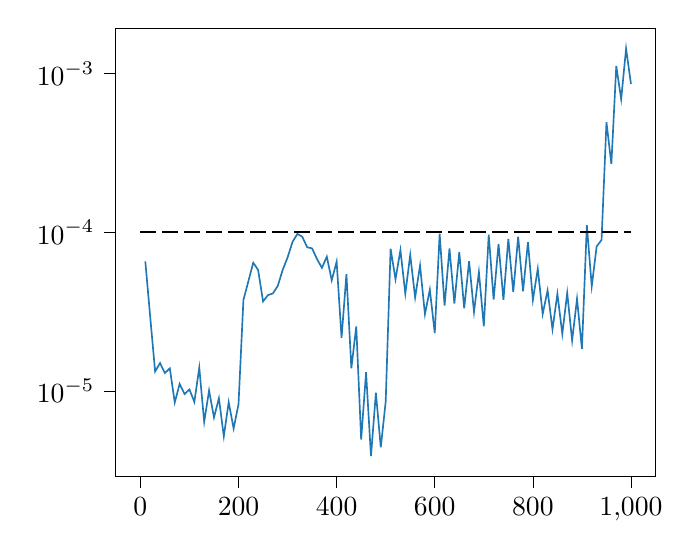
\begin{tikzpicture}

\definecolor{darkgray176}{RGB}{176,176,176}
\definecolor{steelblue31119180}{RGB}{31,119,180}

\begin{axis}[
log basis y={10},
tick align=outside,
tick pos=left,
x grid style={darkgray176},
xmin=-50, xmax=1050,
xtick style={color=black},
y grid style={darkgray176},
ymin=2.88105590692895e-06, ymax=0.00193785870066619,
ymode=log,
ytick style={color=black},
ytick={1e-07,1e-06,1e-05,0.0001,0.001,0.01,0.1},
yticklabels={
  \(\displaystyle {10^{-7}}\),
  \(\displaystyle {10^{-6}}\),
  \(\displaystyle {10^{-5}}\),
  \(\displaystyle {10^{-4}}\),
  \(\displaystyle {10^{-3}}\),
  \(\displaystyle {10^{-2}}\),
  \(\displaystyle {10^{-1}}\)
}
]
\addplot [semithick, steelblue31119180]
table {%
10 6.55859912512824e-05
20 2.92687545879744e-05
30 1.32526329252869e-05
40 1.49589986904175e-05
50 1.29485615616431e-05
60 1.38678942676052e-05
70 8.44683927425649e-06
80 1.10582186607644e-05
90 9.55155428528087e-06
100 1.02034682640806e-05
110 8.51413460623007e-06
120 1.40294660013751e-05
130 6.36767663309001e-06
140 1.00551878858823e-05
150 6.79174581819098e-06
160 8.9875866251532e-06
170 5.16740692546591e-06
180 8.47696082928451e-06
190 5.78804883843986e-06
200 8.24212474981323e-06
210 3.74758456018753e-05
220 4.90443489979953e-05
230 6.42837403574958e-05
240 5.78381441300735e-05
250 3.66622371075209e-05
260 4.0163860830944e-05
270 4.11299370171037e-05
280 4.59189213870559e-05
290 5.79099469177891e-05
300 6.94186528562568e-05
310 8.6939508037176e-05
320 9.77483723545447e-05
330 9.37388758757152e-05
340 8.04420124040917e-05
350 7.92096034274437e-05
360 6.7819157266058e-05
370 5.97074649704155e-05
380 7.02072502463125e-05
390 4.98194567626342e-05
400 6.530387327075e-05
410 2.15935287997127e-05
420 5.44773029105272e-05
430 1.38822933877236e-05
440 2.5478770112386e-05
450 4.93502147946856e-06
460 1.31122396851424e-05
470 3.87334966944763e-06
480 9.72650923358742e-06
490 4.401531896292e-06
500 8.56040423968807e-06
510 7.87561730248854e-05
520 5.05988246004563e-05
530 7.72591884015128e-05
540 4.10577631555498e-05
550 7.20853786333464e-05
560 3.88277840102091e-05
570 6.17690675426275e-05
580 3.04207042063354e-05
590 4.34477624366991e-05
600 2.31486046686769e-05
610 9.80691038421355e-05
620 3.44693471561186e-05
630 7.90198391769081e-05
640 3.55191950802691e-05
650 7.51315819798037e-05
660 3.31502924382221e-05
670 6.57359196338803e-05
680 3.14316203002818e-05
690 5.61431588721462e-05
700 2.55749946518335e-05
710 9.66391744441353e-05
720 3.76222233171575e-05
730 8.4614752267953e-05
740 3.74903029296547e-05
750 9.08605361473747e-05
760 4.19506286561955e-05
770 9.37209042604081e-05
780 4.25264879595488e-05
790 8.67555572767742e-05
800 3.74088558601215e-05
810 5.89142764511053e-05
820 3.05110388580943e-05
830 4.30050386057701e-05
840 2.44616458076052e-05
850 4.09027634304948e-05
860 2.28696044359822e-05
870 4.14731803175528e-05
880 2.07652392418822e-05
890 3.80441488232464e-05
900 1.83884185389616e-05
910 0.000111009663669392
920 4.56731941085309e-05
930 8.14374216133729e-05
940 8.95264456630684e-05
950 0.00049529381794855
960 0.000269378913799301
970 0.00111920747440308
980 0.000691821333020926
990 0.00144140853080899
1000 0.000860700674820691
};
\path [draw=black, semithick, dash pattern=on 5.55pt off 2.4pt]
(axis cs:0,0.0001)
--(axis cs:1000,0.0001);

\end{axis}

\end{tikzpicture}
